\chapter{Missing data: Traffic data}


\section{Data}

Time series on traffic anomalies with missing values.

\begin{figure}[H]
    \centering
    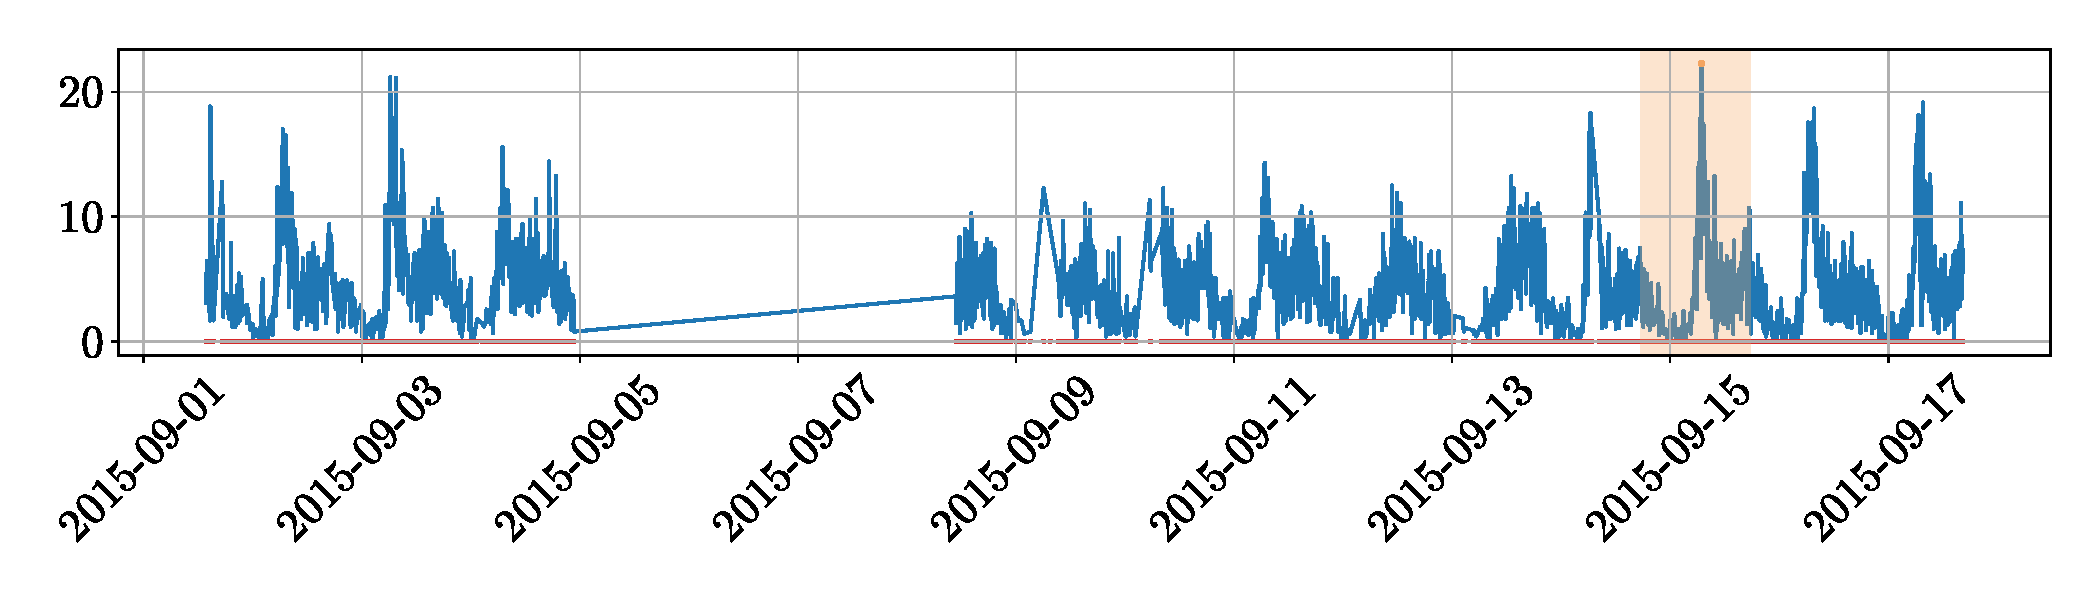
\includegraphics[width=0.8\linewidth]{./img/_md_traffic_data.pdf}
    \caption{
        \parbox[t]{0.7\linewidth}{
            Plot of the data. Straight lines are artifacts of missing values. Red dots below represent the actual data points.
        }
    }
\end{figure}



\section{Preliminaries}

The dataset has sparse indexes (i.e., indexes are non-contiguous) and missing values are represented by gaps. It is necessary to use dense indexes where missing values are explicitly marked as \texttt{NaN}.

\subsection{Resampling / Binning}

\begin{description}
    \item[Resampling / binning] \marginnote{Resampling / binning} 
        Resample the indexes of the dataset so that they have a regular step (e.g., 5 minutes).

        \begin{remark}
            Values that end up in the same bin need to be aggregated (e.g., mean).
        \end{remark}

        \begin{figure}[H]
            \centering
            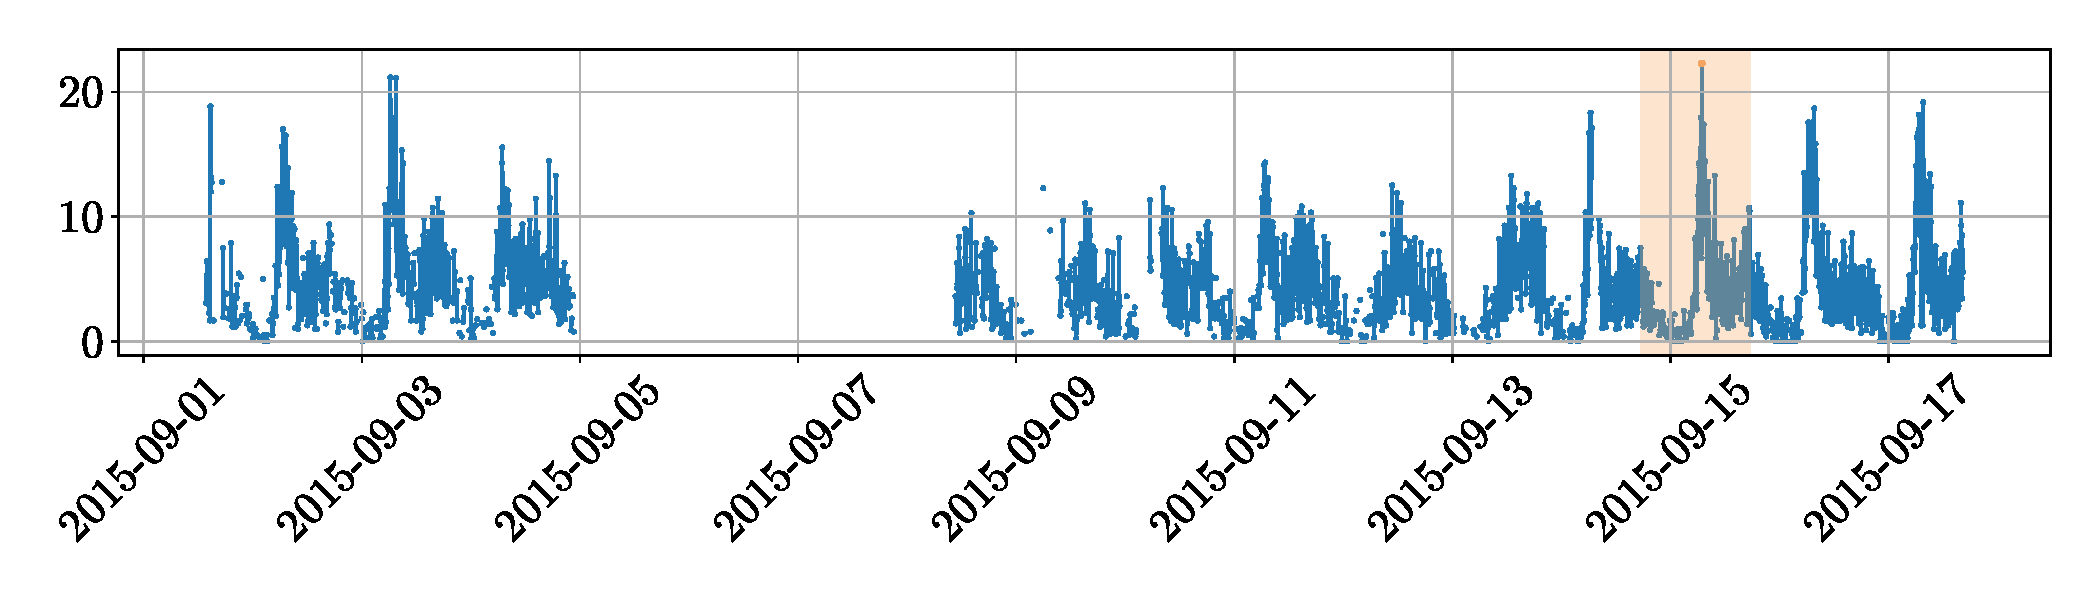
\includegraphics[width=0.8\linewidth]{./img/_md_traffic_resampled.pdf}
            \caption{
                Plot of the resampled data without artifacts
            }
        \end{figure}
\end{description}



\section{Approaches}

\begin{description}
    \item[Benchmark dataset] 
        A portion of known data where some values are artificially removed can be used to evaluate a filling method. As accuracy metric, RMSE can be used.

        \begin{figure}[H]
            \centering
            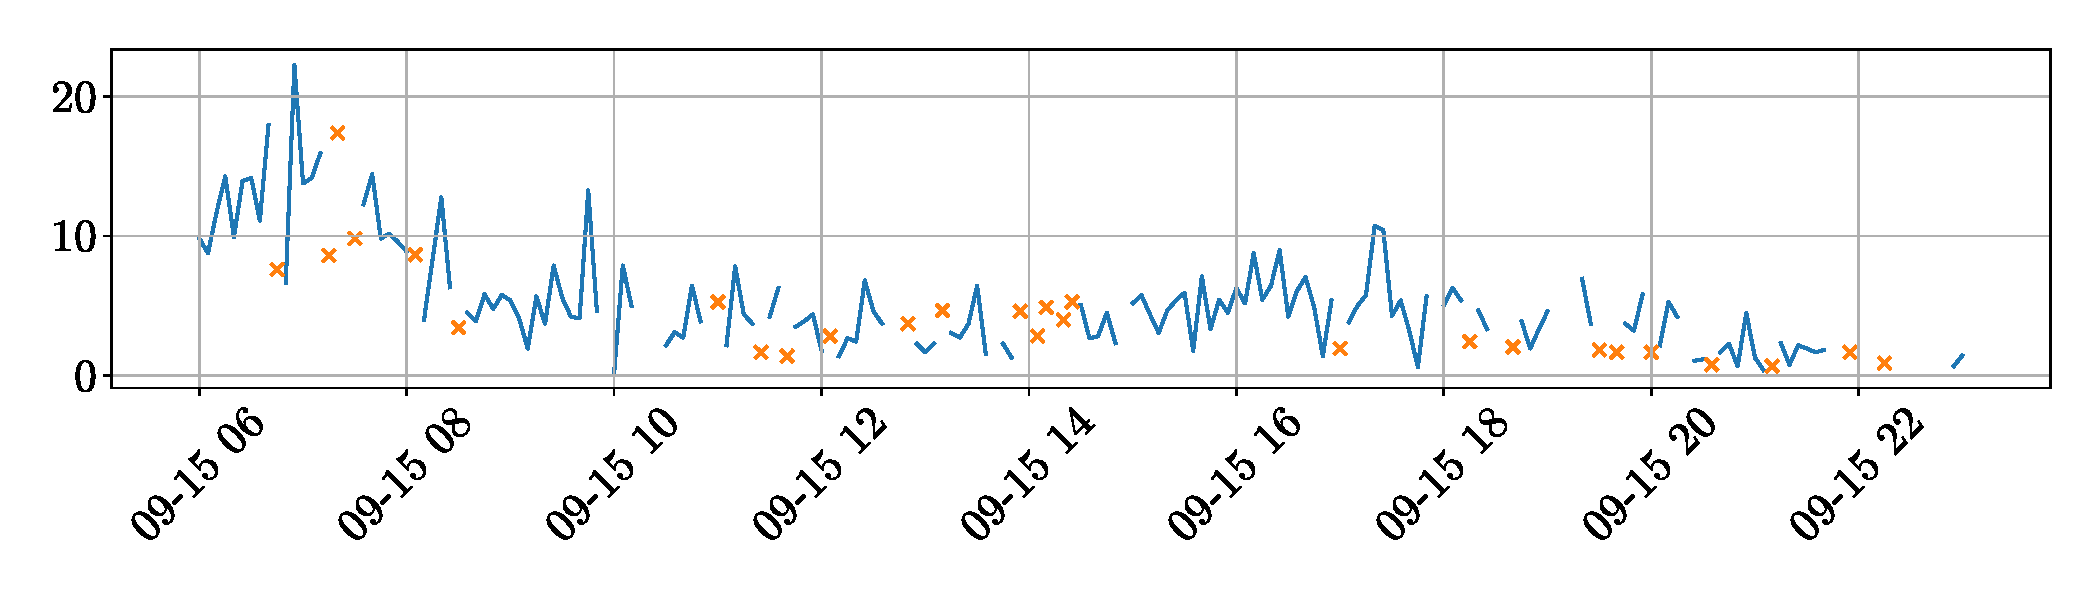
\includegraphics[width=0.8\linewidth]{./img/_md_traffic_eval_data.pdf}
            \caption{Benchmark dataset. Marked points have been artificially removed.}
        \end{figure}
\end{description}


\subsection{Forward/Backward filling}

\begin{description}
    \item[Forward filling] 
        Set the missing value to the last valid observation.

    \item[Backward filling] 
        Set the missing value to the next valid observation.
\end{description}

\begin{remark}
    The idea of this approach is that time series usually have strong local correlation (i.e., some sort of inertia).
\end{remark}

\begin{remark}
    Forward/backward filling tend to work well on low variance portions of the data.
\end{remark}


\subsection{Geometric interpolation}

Interpolate a function to determine missing points. Possible methods are:
\begin{itemize}
    \item Linear,
    \item Nearest value,
    \item Polynomial,
    \item Spline.
\end{itemize}



\begin{remark}
    (R)MSE assumes that the data is normally distributed, independent, and with the same variability at all points. This is not usually true with time series.
\end{remark}

\begin{remark}
    We would like to build an estimator that is:
    \begin{itemize}
        \item At least as powerful as interpolation.
        \item Able to detect the expected variability.
    \end{itemize}
\end{remark}
